%\section{Character of Energy and Electron Transfer Illustrated Using Pairs and Triples of Atoms}
\section{Geometric Influence on ICD and ETMD3  Illustrated Using Pairs and Triples of Atoms}
Approximating every system into pairs and triples of atoms is a very useful
first order approximation to both the investigation of energies and
decay widths of a larger system. Pairs and triples are combinations of
two and three atoms, respectively.
These atoms do not necessarily need to form bonds between each other or
even being close, but they are characterized according to fixed internal
coordinates. Each pair and triple can be described by its properties and
is in first order of approximation independent on further, eventually
present, atoms.

In case of the electronic decay processes one is interested in the
energies of the initial $E_{in}$ and the final states $E_{fin}$ of
the corresponding processes. They can be approximated to be

\begin{align}
 E_{in}  &= SIP(X{in}^\beta)\\
 E_{fin} &= SIP(X_{fin1}^\beta) + SIP(X_{fin2}^\beta) + \frac 1d\\
 E_{sec} &= E_{in} - E_{fin}
\end{align}
where $X_{in}$ denotes the initially ionized atom and
$X_{fin1}$ and $X_{fin2}$ describe the two ionized
atoms in the final state. $/beta$ denotes the decay channel characterized
by the total angular momenta of the ionized atoms in the pairs
and triples and $d$ denotes the interatomic distance between the atoms
$X_{fin1}$ and $X_{fin2}$. The initially ionized atom $X_{in}$ can
coincide with one or both of
the final state atoms
$X_{fin1}$ and $X_{fin2}$. As explained in
section \ref{xyz}, the distribution of the vacancies over the different
atoms determine the kind of electronic decay process. Hence, in an
Auger process all three atoms would coincide, for an ICD $X_{in}$
would coincide with one of $X_{fin1}$ and $X_{fin2}$ and for an \ac{ETMD}3
all ionized states are located on different atoms.

In all considered autoionization processes a second electron
is emitted with the kinetic energy $E_{sec}$. If $E_{sec}<0$, then
the final state energy is higher than the initial state energy and the
process is energetically not accessible.

The decay widths of the pairs and triples can be estimated with
different accuracy, but in general, the total decay width $\Gamma$ of
a system is the sum over the decay widths of all channels $\beta$ for
all possible pairs or triples $i$.

\begin{equation}
  \Gamma = \sum\limits_{i,\beta}\Gamma_{i,\beta}
\end{equation}


\subsection{Influence of the Geometry on ICD processes}
\subsubsection{Geometry Dependence of the ICD Energies}

\begin{figure}[h]
 \centering
 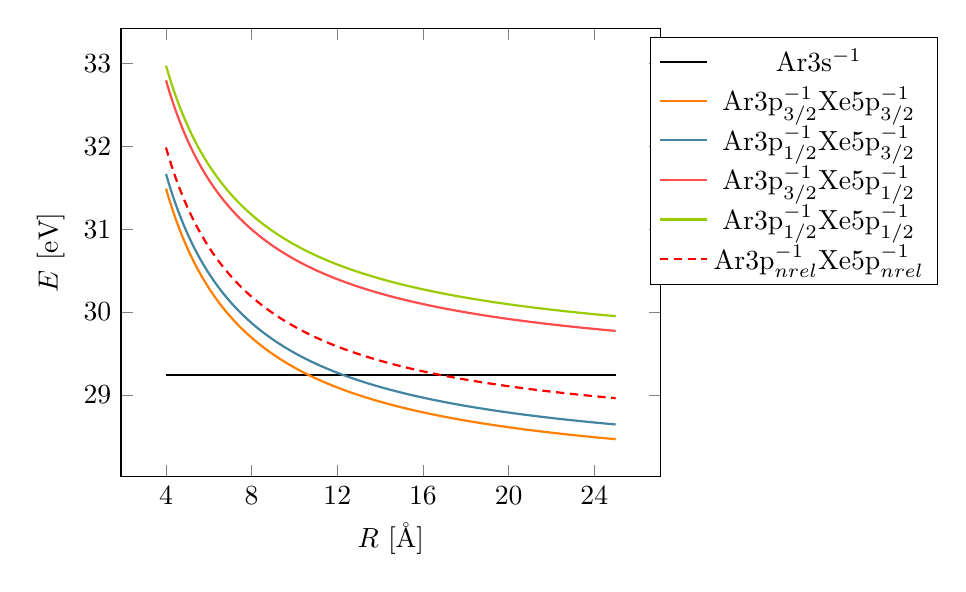
\begin{tikzpicture}
    \begin{axis}[domain=4.0:25,
                 samples = 200,
                 xtick={4.0,8.0,...,24},
                 %xticklabels={$-\pi$,$-\frac \pi 2$,0,$\frac \pi 2$,$\pi$},
                 cycle list name = exotic,
                 legend style={anchor= north west},
                 xlabel={$R$ [\AA]},
                 ylabel={$E$ [eV]}
                 ]
      \addplot+[
                mark = none,
                black,
                thick
               ]
               {29.239};
      \addlegendentry{Ar3s$^{-1}$};
      \addplot+[
                mark = none,
                thick
               ]
               {15.7596 + 12.1298 + 14.39964 / x};
      \addlegendentry{Ar3p$_{3/2}^{-1}$Xe5p$_{3/2}^{-1}$};
      \addplot+[
                mark = none,
                thick
               ]
               {15.9371 + 12.1298 + 14.39964 / x};
      \addlegendentry{Ar3p$_{1/2}^{-1}$Xe5p$_{3/2}^{-1}$};
      \addplot+[
                mark = none,
                thick
               ]
               {15.7596 + 13.4363 + 14.39964 / x};
      \addlegendentry{Ar3p$_{3/2}^{-1}$Xe5p$_{1/2}^{-1}$};
      \addplot+[
                mark = none,
                thick
               ]
               {15.9371 + 13.4363 + 14.39964 / x};
      \addlegendentry{Ar3p$_{1/2}^{-1}$Xe5p$_{1/2}^{-1}$};
      \addplot+[
                mark = none,
                thick
               ]
               {15.8188 + 12.5653 + 14.39964 / x};
      \addlegendentry{Ar3p$_{nrel}^{-1}$Xe5p$_{nrel}^{-1}$};
      %\draw[] (axis cs:\pgfkeysvalueof{/pgfplots/xmin},29.239) -- (axis cs:\pgfkeysvalueof{/pgfplots/xmax},29.239);
    \end{axis}
\end{tikzpicture}

 \caption{}
 %\label{}
\end{figure}

\subsubsection{Geometry Dependence of the ICD Decay Widths}
